% -*- TeX-command-extra-options: "-shell-escape"; -*-
\documentclass[
% convert={density=1200,size=1080x800,outext=.png},
tikz]{standalone}
\usepackage{amsmath}
\usetikzlibrary{matrix}
\usetikzlibrary{angles, quotes}
\usetikzlibrary{intersections}
% \usetikzlibrary{arrows.meta}
\begin{document}
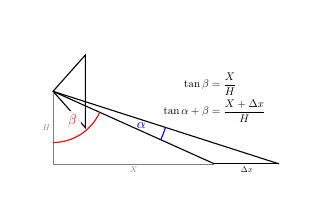
\begin{tikzpicture}

  \matrix (grid) [matrix of nodes, transparent=1]
  {
    1 & 2 & 3 & 4 & 5 & 6 & 7 & 8 \\
    1 & 2 & 3 & 4 & 5 & 6 & 7 & 8 \\
    1 & 2 & 3 & 4 & 5 & 6 & 7 & 8 \\
    1 & 2 & 3 & 4 & 5 & 6 & 7 & 8 \\
  };

  % camera
  \draw[name path=lens] (grid-2-1.center)
  to (grid-1-2.center)
  to (grid-3-2.center)
  to cycle;

  % height, x, \Delta x
  \draw[gray, very thin] (grid-2-1.center) to node[left, scale=0.3] {$H$} (grid-4-1.center);
  \draw[gray, very thin] (grid-4-1.center) to node[below, scale=0.3] {$X$} (grid-4-6.center);
  \draw (grid-4-6.center) to node[below, scale=0.3] {$\Delta x$} (grid-4-8.center);

  % projection lines
  \draw (grid-2-1.center) to (grid-4-6.center);
  \draw (grid-2-1.center) to (grid-4-8.center);

  % angle \alpha
  \draw[blue, opacity=0] (grid-4-6.center) coordinate (A) to (grid-2-1.center) coordinate (B) to (grid-4-8.center) coordinate (C)
  pic ["$\alpha$"{scale=0.5, opacity=1}, draw, solid, angle radius=1.5cm, angle eccentricity=0.8, opacity=1] {angle};

  % angle \beta
  \draw[red, opacity=0] (grid-4-1) coordinate (A)
  to (grid-2-1) coordinate (B)
  to (grid-4-6) coordinate (C)
  pic["$\beta$"{scale=0.5, opacity=1, fill=white, fill opacity=0.9},
      opacity=1, draw, solid, angle radius=0.65cm, angle eccentricity=0.7] {angle};


  \node[scale=0.4, anchor=center] at (grid-2-6) {
\begin{minipage}{3cm}\begin{align*}
                       \tan{\beta} &= \frac{X}{H} \\
                       \tan{\alpha + \beta} &= \frac{X+\Delta x}{H}
  \end{align*}\end{minipage}};
\end{tikzpicture}
\end{document}
